\subsection{Mediciones}

Realizar una medición de performance \emph{rigurosa} es más difícil de lo 
que parece. 
En este experimento deberá realizar distintas mediciones de performance 
para verificar que sean buenas mediciones.

En un sistema ``ideal'' el proceso medido corre solo, sin ninguna 
interferencia de agentes externos. 
Sin embargo, una PC no es un sistema ideal. 
Nuestro proceso corre junto con decenas de otros, tanto de usuarios como 
del sistema operativo que compiten por el uso de la CPU. 
Esto implica que al realizar mediciones aparezcan ``ruidos'' o 
``interferencias'' que distorsionen los resultados.

El primer paso para tener una idea de si la medición es buena o no, 
es tomar varias muestras. 
Es decir, repetir la misma medición varias veces.
Luego de eso, es conveniente descartar los outliers
\footnote{en español, valor atípico: \url{http://es.wikipedia.org/wiki/Valor_atípico}}, 
que son los valores que más se alejan del promedio. 
Con los valores de las mediciones resultantes se puede calcular el promedio 
y también la varianza, que es algo similar el promedio de las distancias al 
promedio\footnote{en realidad, elevadas al cuadrado en vez de tomar el módulo}.

Las fórmulas para calcular el promedio $\mu$ y la varianza $\sigma^2$ son

$$
\mu = \frac{1}{n}\sum_{i=1}^{n} x_i \qquad \sigma^2 = \frac{\displaystyle\sum_{i=1}^{n}(x_i - \mu)^2} {n}
$$
%------------------------------------------

\subsection{Filtro \textit{cropflip}}

Programar el filtro \textit{cropflip} en lenguaje C y luego en ASM haciendo 
uso de las instrucciones vectoriales (\textbf{SSE}).

% ******************************************************************************
\vspace*{0.3cm} \noindent
\textbf{Experimento 1.1 - análisis el código generado}

En este experimento vamos a utilizar la herramienta \verb|objdump| para 
verificar como el compilador de C deja ensamblado el código C.

Ejecutar 
\begin{codesnippet}
\begin{verbatim}
objdump -Mintel -D cropflip_c.o
\end{verbatim}
\end{codesnippet}

¿Cómo es el código generado? 
Indicar\\
\begin{inparaenum}[\itshape a\upshape)]
    \item Por qué cree que hay otras funciones además de \verb|cropflip_c|
    \item Cómo se manipulan las variables locales
    \item Si le parece que ese código generado podría optimizarse
\end{inparaenum}\\
\\
\indent Muchas de las funciones generadas se agregan al compilar usando parámetros de debugging.\\ 
\indent El cambio que puede notarse a simple vista es que el tamaño del código generado con optimización es considerablemente menor al generado sin optimizaciones, un 34\% menor. Por otro lado, calcula una única vez la posición de la cual deberá leer el pixel a procesar, ya que es una operación que se realiza cuatro veces por cada lectura y escritura de un pixel. \\
\indent El c\'odigo optimizado también disminuye el uso del stack para variables locales y en su lugar utiliza registros, por esa razón necesita armar el stackframe y pushear los registros que la convención C pide preservar. Esto no se da en el c\'odigo sin optimizar, todas las variables locales se guardar en el stack, se asignan a algún registro libre al momento de usarla y luego vuelve a ser guardada en el stack. Si bien la cantidad de accesos a memoria es sustencialmente mayor en el c\'odigo sin optimizar por el hecho de que se accede constantemente a las variables locales alojadas en el stack, también hay que considerar que al haber tantos accesos al stack el hit-rate de la caché debería ser bastante alto, agilizando la lectura, no así la escritura. \\

% ******************************************************************************
%\newpage
\vspace*{0.3cm} \noindent
\textbf{Experimento 1.2 - optimizaciones del compilador}

Compile el código de C con flags de optimización. Por ejemplo, pasando el flag 
\verb|-O1|\footnote{agregando este flag a \texttt{CCFLAGS64} en el makefile}. 
Indicar\\
\begin{inparaenum}
    \item Qué optimizaciones observa que realizó el compilador\\
    \item Qué otros flags de optimización brinda el compilador\\
    \item Los nombres de tres optimizaciones que realizan los compiladores.\\
\end{inparaenum}\\
\\
\indent GCC provee un arsenal de optimizaciones disponibles para que podamos usar cuando lo creamos conveniente, asímismo provee unos flags para poder compilar el código con un conjunto de optimizaciones, estos son O1, O2, O3, Os, entre otros. O1, O2 y O3 son optimizaciones generales no agresivas, es decir, no deberían modificar el funcionamiento del programa. Otras optimizaciones podrían asumir que todas las operaciones aritméticas son sin signo o que están bien implementadas y no es necesario chequear la consistencia de los resultados (fno-math-errno). Estas optimizaciones tienen como objetivo mejorar la performance del programa, sin embargo Os tiene como objetivo reducir el tamaño del ejecutable, es decir, activa todas las optimizaciones que contribuyen a reducir la cantidad de instrucciones regardless del impacto que esto pueda tener en la performance del programa. \\
\indent Concretamente al activar las optimizaciones O3 en cropflip el cambio más notorio es que GCC utiliza instrucciones SSE para procesar 4 pixels por iteración, lo cual le brinda un boost de velocidad impresionante. Además de haberse reducido la cantidad de instrucciones. \\
\\
%----------------------------------------------
\vspace*{0.3cm} \noindent
\textbf{Experimento 1.3 - calidad de las mediciones}

\begin{enumerate}
    \item Medir el tiempo de ejecución de cropflip 10 veces. Calcular el promedio y la varianza. Consideraremos outliers a los 2 mayores tiempos de ejecución de la medicion y también a los 2 menores, por lo que los descartaremos. Recalcular el promedio y la varianza después de hacer este descarte. Realizar un gráfico que presente estos dos últimos items.\\
\\
Luego de ejecutar 10 veces el filtro Cropflip obtuvimos los siguientes resultados: \\
\\
    	\begin{tabular}[c]{|c|c|c|}
	\hline
		\textbf{ASM} & \textbf{C}\\
		\hline
70.925 &	1.152.187\\
		\hline
70.521 &	1.151.544\\
		\hline
32.859 &	761.937\\
		\hline
43.720 &	649.248\\
		\hline
64.236 &	1.152.847\\
		\hline
70.793 &	1.153.061\\
		\hline
71.271 &	1.152.765\\
		\hline
44.616 &	1.152.798\\
		\hline
56.124 &	725.420\\
		\hline
71.775 &	1.155.718\\
		\hline
	\textbf{Esperanza}	\\
		\hline
59.684 & 1.020.752,5 \\
		\hline
		\textbf{Desvío est\'andar}	\\
		\hline
13.720,5329 & 203.626,443 \\
		\hline
	\end{tabular}\\\\


	El cuadro denota la cantidad de ciclos de clock utilizada por cada ejecuci\'on del programa. \\
	\\
	Se puede apreciar que la esperanza (promedio de las mediciones) bajo Lenguaje C es notablemente mayor para las diez mediciones llevadas a cabo. Adem\'as poseen una desviaci\'on est\'andar tambi\'en mayor. La desviación estándar mide el grado de dispersión o variabilidad, por lo que demuestra menor estabilidad en las mediciones bajo Lenguaje C. Por lo tanto podemos afirmar que bajo el contexto de nuestras mediciones el tiempo de ejecuci\'on del mismo programa en lenguaje ASM posee un tiempo de c\'omputo menor. \\
\\	
	
	Luego de eliminar los dos valores m\'as altos y los dos valores m\'as bajos, recalculamos obteniendo los siguientes datos: \\
	\textbf{Esperanza}: 62.869,16667(ASM) y 1.087.346,333(C)\\
	\textbf{Desvío est\'andar}:	9.719,205547(ASM) y 145.528,2027(C)\\

	Se puede ver que al eliminar los outliers, el valor de la esperanza aumenta en ambos casos. Al haber hecho una medici\'on tan peque\~na, los c\'alculos de la esperanza no son tan estables y no son los m\'as ``parecidos'' a la realidad. Lo que s\'i ocurre es que al eliminar los valores mas alejados del promedio, como era de esperar, disminuye la desviaci\'on est\'andar al haber dejado s\'olo las mediciones m\'as cercanas entre s\'i.\\

\begin{figure}[h!]
  \begin{center}
	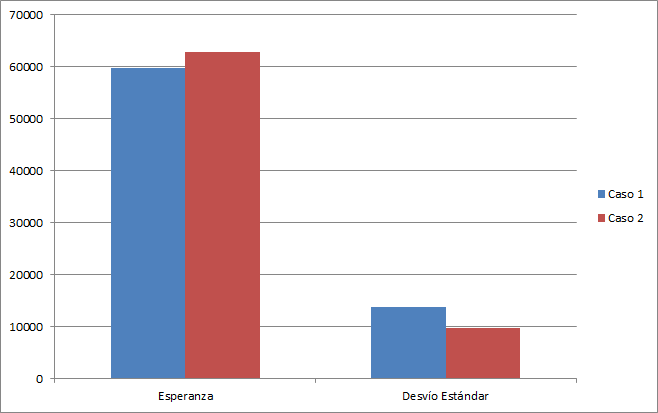
\includegraphics[width=0.7\textwidth]{imagenes/asm1}
	\caption{Assembler}
      \end{center}
\end{figure}

\newpage 
\begin{figure}[h!]
  \begin{center}
%	\label{nombreparareferenciar}
	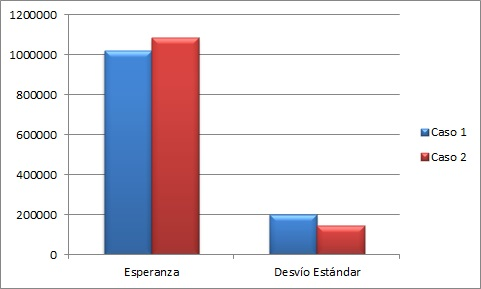
\includegraphics[width=0.7\textwidth]{imagenes/C1}
	\caption{C}
  \end{center}
\end{figure}


\indent Siendo el Caso 1 las mediciones de esperanza y Desvío est\'andar para todos los casos de test y el Caso 2 las mediciones sin tener en cuenta los cuatro outliers.\\

\bigskip
    \item Implementar un programa en C que no haga más que ciclar infinitamente sumando 1 a una variable. Lanzar este programa tantas veces como \emph{cores lógicos} tenga su procesador. Medir otras 10 veces mientras estos programas corren de fondo. Realizar los mismos casos de experimentaci\'on que en el ejercicio anterior.\\
\end{enumerate}
Los resultados obtenidos en esta experimentaci\'on fueron menores que los anteriores: \\
\\       
        \begin{tabular}[c]{|c|c|c|}
	\hline
		\textbf{ASM} & \textbf{C}\\
		\hline
33.585 &	542.928 \\
\hline
33.798 &	544.155 \\
\hline
33.402 &	544.857 \\
\hline
33.228 &	543.687 \\
\hline
33.159 &	543.252 \\
\hline
33.441 &	543.324 \\
\hline
34.089 &	544.224 \\ 
\hline
33.768 &	760.359 \\ 
\hline
34.563 &	542.448 \\
\hline
34.473 &	542.982 \\
\hline
		\textbf{Esperanza}	\\
		\hline
33.750,6 & 565.221,6	\\		
		\hline
		\textbf{Desvío est\'andar}	\\
		\hline
465,49 & 65.049,34\\
		\hline
	\end{tabular}\\\\
	Luego de eliminar los dos valores m\'as altos y los dos valores m\'as bajos, recalculamos obteniendo los siguientes datos: \\
	\textbf{Esperanza}: 33.680,5 (ASM) y 543.604(C)\\
	\textbf{Desvío est\'andar}:	235,364 (ASM) y 462,615(C)\\
	Ac\'a tambi\'en se puede apreciar que al eliminar los outliers, el Desvío est\'andar disminuye su valor. \\

Se puede observar que las mediciones mejoran con la ejecuci\'on del ciclo infinito de fondo, esto se debe a que fue ejecutado en una computadora con un procesador i5. La familia ix de intel varía la frecuencia del clock de acuerdo al uso requerido. Por eso cuando ejecutamos los sumadores puede llegar a tardar menos que en la versi\'on sin ellos.\\
\\

Por este motivo, volvimos a ejecutar este caso una mayor cantidad de veces para que el procesador no modifique la frecuencia de clock, obteniendo los siguientes resultados: \\
\begin{itemize}
\item[$\bullet$] Teniendo en cuenta todas las mediciones realizadas: \\
\textbf{Esperanza:} 434.338,4653(ASM) y 12.183.006,91(C). \\
\textbf{Desv\'io est\'andar:} 659,0435989(ASM) y 8.230.692,407(C).
\item[$\bullet$] Eliminando los \textit{outliers}: \\
\textbf{Esperanza:} 270.056,844(ASM) y 9.525.801,857(C). \\
\textbf{Desv\'io est\'andar:} 524,7013438(ASM) y 8.648.990,473(C).
\end{itemize}

\begin{figure}[h!]
  \begin{center}
	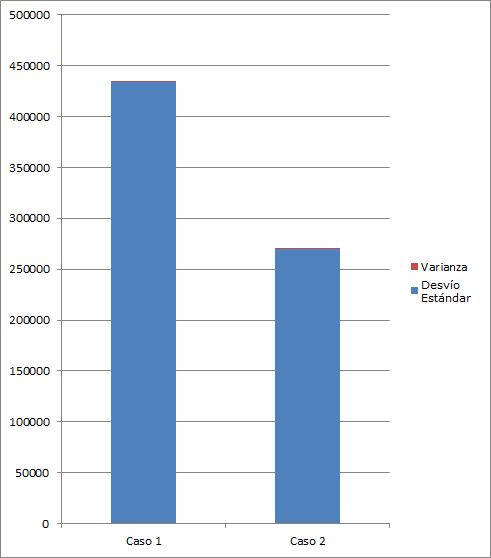
\includegraphics[width=0.7\textwidth]{imagenes/perdidaASM}
	\caption{Assembler}
  \end{center}
\end{figure}

\newpage
\begin{figure}[h!]
  \begin{center}
	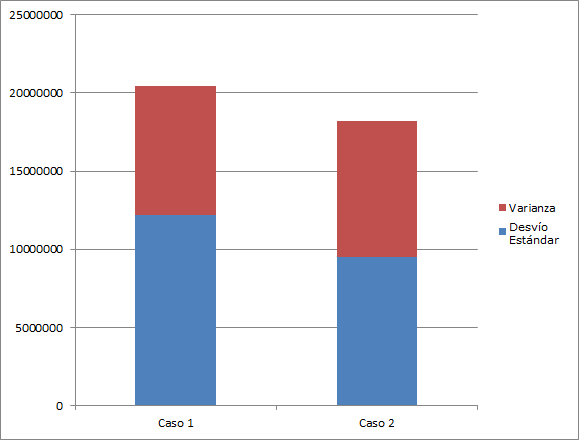
\includegraphics[width=0.7\textwidth]{imagenes/perdidaC}
	\caption{C}
  \end{center}
\end{figure}

\indent \textit{Siendo el Caso 1 las mediciones de esperanza y Desvío est\'andar para todos los casos de test y el Caso 2 las mediciones sin tener en cuenta los cuatro outliers.}\\

Tal como se puede apreciar en los gr\'aficos, la varianza en Assembler es casi despreciable pero la de C no lo es. Sin embargo, ahora s\'i ocurre algo m\'as intuitivo que es que aumentaron los valores de la esperanza en proporciones notables. \\
\\

 \bigskip
\textit{A partir de aquí todos los experimentos de mediciones deberán hacerse igual 
que en el presente ejercicio: tomando 10 mediciones, luego descartando 
outliers y finalmente calculando promedio y Desvío est\'andar.}\\
\\
Decidimos: \\

Realizar 12000 mediciones por experimento, eliminando los primeros dos mil quinientos casos que hayan llevado menos ciclos de clock y los dos mil quinientos casos que hayan llevado la mayor cantidad de ciclos de clock. 

Lo determinamos de esta manera, ya que dejar dos mediciones afuera, como dice el enunciado, no tiene influencia en los c\'alculos de la esperanza y la varianza para muestras tan grandes. 

Luego de experimentar distintas cantidades de casos de testeo, notamos que elegir 7000 valores pertenecientes a la franja del medio de los 12000 es una soluci\'on lo suficientemente estable, por lo cual es la que llevamos a cabo. \\
\\
% ******************************************************************************
\newpage
\noindent\textbf{Experimento 1.4 - secuencial vs. vectorial}

En este experimento deberá realizar una medición de las diferencias de 
performance entre las versiones de C y ASM (el primero con -O0, -O1, -O2 y -O3) 
y graficar los resultados. \\
\\
El siguiente gr\'afico indica la esperanza de la cantidad de ciclos de clock que toma ejecutar el filtro Cropflip con los par\'ametros 404 404 4 4 en ASM y en C variando los flags de o0 a o3. \\
Reflejando las siguientes magnitudes: \\
\\
 \begin{tabular}[c]{|c|c|c|}
	\hline
		 & Esperanza & Desv\'io est\'andar\\
		\hline
C -o0 & 6.761.044,5 & 131,463 \\
\hline
C -o1 & 1.300.109 & 53,447 \\
\hline
C -o2 & 1.227.102,5 & 50,143\\
\hline
C -o3 & 266.688 & 0,287 \\
\hline
ASM & 362.232 & 2,079\\
\hline
	\end{tabular}\\\\

\begin{figure}[h!]
  \begin{center}
	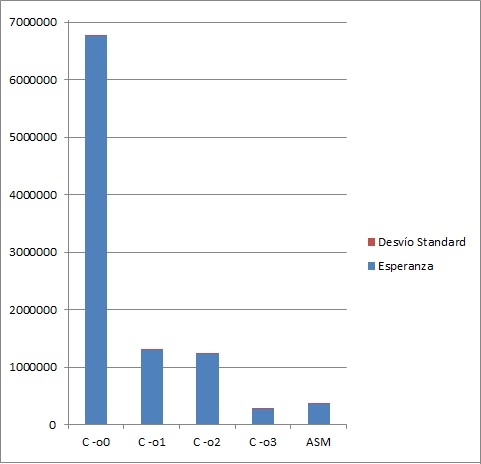
\includegraphics[width=0.7\textwidth]{imagenes/14.jpg}
  \end{center}
\end{figure}


Se puede observar que la varianza es casi despreciable considerando el valor de la esperanza. Adem\'as, es notorio c\'omo el correr el programa con la orden de -o0 no efect\'ua ninguna optimizaci\'on. Tambi\'en se puede observar que el c\'odigo corrido en C bajo el comando de -o3 tiene una esperanza menor a la del c\'odigo Assembler. Esto se debe a que el flag de optimizaci\'on -o3 lo que hace es utilizar instrucciones SSE para procesar 4 pixels por iteración, lo cual le brinda un boost de velocidad mucho mayor. Además de haberse reducido la cantidad de instrucciones. Tal cual lo explicado anteriormente. Y por este motivo, es una buena optimizaci\'on para el c\'odigo.

\newpage

% ******************************************************************************
\vspace*{0.3cm} \noindent
\textbf{Experimento 1.5 - cpu vs. bus de memoria}

Se desea conocer cual es el mayor limitante a la
performance de este filtro en su versión ASM.

¿Cuál es el factor que limita la performance en este caso?
En caso de que el limitante fuera la intensidad de cómputo, entonces 
podrían agregarse instrucciones que realicen accesos a memoria extra y la
performance casi no debería sufrir. 
La inversa puede aplicarse, si el limitante es la cantidad de accesos a memoria.
\footnote{también podría pasar que estén más bien balanceados y que agregar
cualquier tipo de instrucción afecte sensiblemente la performance}
	
Realizar un experimento, agregando 4, 8 y 16 instrucciones aritméticas 
(por ej \verb|add rax, rbx|) analizando como varía el tiempo de ejecución.
Hacer lo mismo ahora con instrucciones de acceso a memoria, haciendo 
mitad lecturas y mitad escrituras (por ejemplo, agregando dos 
\verb|mov rax, [rsp]| y dos \verb|mov [rsp+8], rax|).\footnote{Notar que en el caso de acceder a \texttt{[rbp]} o \texttt{[rsp+8]} probablemente haya siempre hits en la cache, por lo que la medición no será de buena calidad. Si se le ocurre la manera, realizar accesos a otras direcciones alternativas.}
	
Realizar un único gráfico que compare:
\begin{inparaenum}
    \item La versión original
    \item Las versiones con más instrucciones aritméticas
    \item Las versiones com más accesos a memoria
\end{inparaenum}
\\
Acompañar al gráfico con una tabla que indique los valores graficados. \\
\\
Las instrucciones aritm\'eticas usadas son:  \emph{add eax,8 sub eax 8} repetidas la cantidad de veces necesitada y los accesos a memoria realizados fueron siempre a la imagen fuente o la de destino, ya que tenemos la certeza de poseer el permiso para acceder a esas direcciones.\\
\\
 \begin{tabular}[c]{|c|c|c|}
	\hline
		Cropflip & Esperanza & Desv\'io est\'andar\\
		\hline
Versi\'on com\'un & 157.236,897 & 5.334,414 \\
\hline
Con 4 instrucciones aritméticas & 183.968,425 & 8.391,506 \\
\hline
Con 8 instrucciones aritméticas & 225.991,244 & 7.729,428 \\
\hline
Con 16 instrucciones aritméticas & 707.857,067 & 12.756,322 \\
\hline
Con 4 accesos a memoria & 281.032,176 & 11.258,907 \\
\hline
Con 8 accesos a memoria & 352.370,777 & 14.353,789 \\
\hline
Con 16 accesos a memoria & 342.023,334 & 12.136,799 \\
\hline
	\end{tabular}\\\\
\\

\begin{figure}[h!]
  \begin{center}
	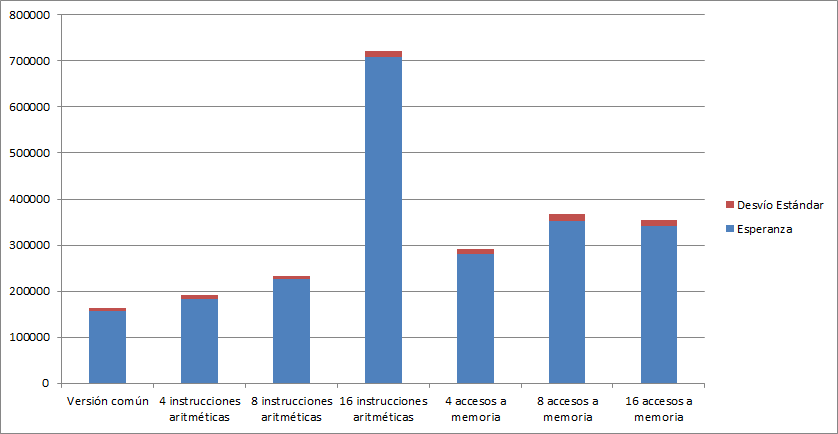
\includegraphics[width=0.8\textwidth]{imagenes/15}
  \end{center}
\end{figure}

Como era de esperar, la versión original es la que menos tiempo demanda. Al agregarle 4 y 8 instrucciones aritméticas, se observa un incremento gradual que se condice con la cantidad de instrucciones. Al agregarle 16 instrucciones se puede observar un pico en la medición, el cual nos hace pensar que la forma en que se aumenta el tiempo de ejecución no es lineal respecto de la cantidad instrucciones, aunque no hay que omitir que de 4 a 8 y a 16 se va incrementando en potencia de dos (lo cual tampoco es lineal).  En el caso de los accesos a memoria no sucede lo mismo que lo descripto anteriormente, cuando se agregan 4 accesos aumenta la cantidad de tiempo respecto de la original, también es así cuando se realizan 8 accesos, pero al realizar 16 accesos en nuestras mediciones disminuye el valor de su esperanza e incluso el de la varianza. Esto no es un indicador con el que podamos afirmar que siempre al realizar 16 accesos a memoria va a tardar menos que al hacer 8. Lo que intuímos que puede suceder es que, el aumento tampoco acá es lineal y para ese intervalo (8,16) el incremento es paulatino. Tampoco hay que dejar de lado que toda medición contiene cierto error y no es exacta y que, a pesar de haber eliminado los outliers, el resultado obtenido se aleje un poco de la ``realidad''.

% ------------------------------------------------------------------------------
  \newpage
\subsection{Filtro \textit{Sierpinski}}

Programar el filtro \textit{Sierpinski} en lenguaje C y en en ASM haciendo 
uso de las instrucciones vectoriales (\textbf{SSE}).

% ******************************************************************************
\vspace*{0.3cm} \noindent
\textbf{Experimento 2.1 - secuencial vs. vectorial}

Analizar cuales son las diferencias de performace entre las versiones de C 
y ASM de este filtro, de igual modo que para el experimento 1.4. \\
\\
El gr\'afico a continuaci\'on indica la esperanza y el desv\'io est\'andar de la cantidad de ciclos de clock que toma ejecutar el filtro Sierpinski en ASM y en C variando los flags de o0 a o3. \\
Reflejando las siguientes magnitudes: \\
\\
 \begin{tabular}[c]{|c|c|c|}
	\hline
		 & Esperanza & Desv\'io est\'andar\\
		\hline
C -o0 & 28.801.586,5 & 78,016 \\
\hline
C -o1 & 21.395.732 & 78,447 \\
\hline
C -o2 & 14.231.758 & 116,445 \\
\hline
C -o3 & 14.229.650 & 116,022 \\
\hline
ASM & 3.661.626 & 115,583 \\
\hline
	\end{tabular}\\\\
\\

\begin{figure}[h!]
  \begin{center}
	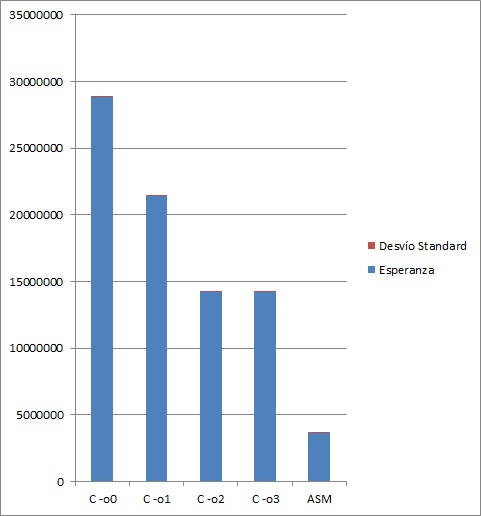
\includegraphics[width=0.7\textwidth]{imagenes/21.jpg}
  \end{center}
\end{figure}

Aqu\'i tambi\'en el valor del desv\'io est\'andar es despreciable. Donde correr el c\'odigo en C bajo el comando -o0 sigue siendo el caso con mayor esperanza (peor caso) y adem\'as la esperanza del c\'odigo Assembler es menor a la del c\'odigo C con -o3. Las optimizaciones -o2 y -o3 arrojan resultados similares, ambos por encima de los valores en ASM. En este caso, notablemente es m\'as eficaz el filtro programado en Assembler.



% ******************************************************************************
\newpage
\vspace*{0.3cm} \noindent
\textbf{Experimento 2.1 - cpu vs. bus de memoria}

¿Cuál es el factor que limita la performance en este filtro?
Repetir el experimento 1.5 para este filtro. \\

Las instrucciones utilizadas son las mismas que en el caso anterior, lo mismo con los accesos a memoria.\\
\\
 \begin{tabular}[c]{|c|c|c|}
	\hline
		 & Esperanza & Desv\'io est\'andar\\
		\hline
Versi\'on com\'un & 2.936.302,152 & 26.416,331 \\
\hline
Con 4 instrucciones aritméticas & 2.961.773,596 & 47.749,307 \\
\hline
Con 8 instrucciones aritméticas & 2.940.553,343 & 59.912,727 \\
\hline
Con 16 instrucciones aritméticas & 3.031.280,298 & 37.499,415 \\
\hline
Con 4 accesos a memoria & 2.919.253,679 & 57.697,386 \\
\hline
Con 8 accesos a memoria & 2.936.432,138 & 56.870,171 \\
\hline
Con 16 accesos a memoria & 3.051.926,505 & 40.964,812 \\
\hline
	\end{tabular}\\\\


\begin{figure}[h!]
  \begin{center}
	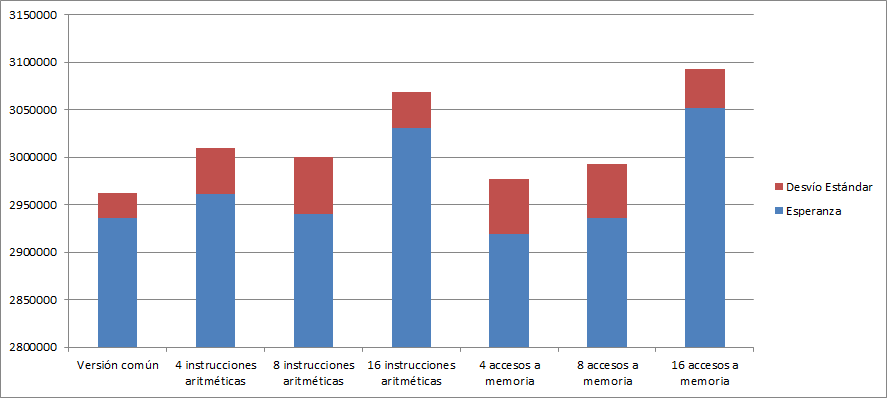
\includegraphics[width=0.9\textwidth]{imagenes/21B}
  \end{center}
\end{figure}

En este caso, lo primero que nos parece necesario destacar es la magnitud del desv\'io est\'andar en todos los casos; son desv\'ios est\'andar grandes, dados los valores de la esperanza. Esto nos indica que los resultados de las mediciones obtenidas pueden no ser tan precisos como necesitamos ya que hay mucha dispersi\'on.\\

Teniendo en cuenta lo mencionado arriba, se puede explicar porqu\'e al sumarle al programa 4 instrucciones aritm\'eticas aumenta la cantidad de tiempo necesaria respecto de la versi\'on original, al igual que al sumarle 16 instrucciones pero no sucede lo mismo en el caso de las 8 instrucciones, ya que la esperanza es muy cercana num\'ericamente a la versi\'on original. Observando el gr\'afico, queda expuesto notablemente que el desv\'io est\'andar de este caso es el mayor (siendo m\'as del doble que en la versi\'on com\'un). Asumimos que en el caso ``ideal'' el crecimiento es paulatino y el tiempo necesario para ejecutar las 8 instrucciones queda por encima del caso anterior y por debajo del siguiente.\\

En el caso de los accesos a memoria, si bien tambi\'en presentan un notoriamente elevado valor de desv\'io est\'andar para todos los casos, el comportamiento es m\'as intuitivo. Se puede apreciar en el gr\'afico que el incremento del tiempo es acorde al aumento de los accesos a memoria y se da de manera pareja sin presentar ning\'un tipo de ``pico''.


\newpage

\subsection{Filtro \textit{Bandas}}

Programar el filtro \textit{Bandas} en lenguaje C y en en ASM haciendo uso de 
las instrucciones vectoriales (\textbf{SSE}).

% ******************************************************************************
\vspace*{0.3cm} \noindent
\textbf{Experimento 3.1 - saltos condicionales}

Se desea conocer que tanto impactan los saltos condicionales en el código 
de filtro Bandas con \verb|-O1| (la versión en C).\\
Para poder medir esto de manera aproximada, remover el código
que detecta a que banda pertenece cada pixel, dejando
sólo una banda.
Por más que la imagen resultante no sea correcta, será posible tomar una
medida aproximada del impacto de los saltos condicionales.
Analizar como varía la performance. \\
\\
En la siguiente figura se ve c\'omo var\'ia la esperanza y el desv\'io est\'andar entre dos corridas de C con el flag -o1 ambas, el Caso 1 es la versión original y el Caso 2 es comentando la guarda de las bandas:

\begin{figure}[h!]
  \begin{center}
	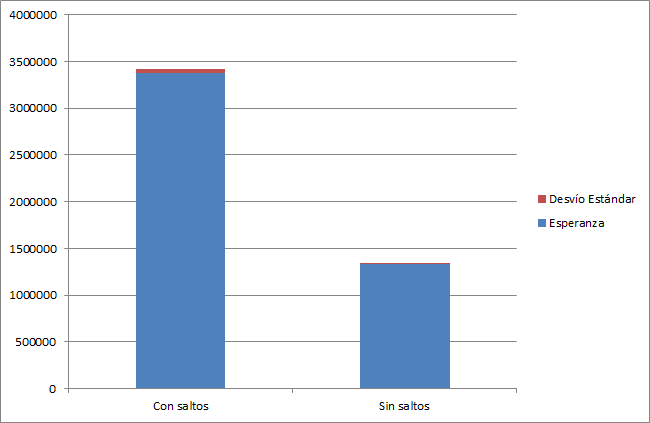
\includegraphics[width=0.7\textwidth]{imagenes/saltitos}
  \end{center}
\end{figure}

Los valores del gr\'afico son:\\

Versi\'on original: esperanza de 3.374.834,128	y varianza de 48.256,45868.\\

Versi\'on sin guarda: esperanza de 1.333.624,786 y varianza de 2.545,912732.\\
\\
	

En el gr\'afico anterior se puede ver que la influencia de los saltos condicionales es notable, ya que disminuye de manera notable la esperanza, siendo en ambos casos la varianza peque\~na. \\

% ******************************************************************************
\newpage
\vspace*{0.3cm} \noindent
\textbf{Experimento 3.2 - secuencial vs. vectorial}

Repetir el experimento 1.4 para este filtro. \\
\\
El siguiente gr\'afico indica la esperanza de la cantidad de ciclos de clock que toma ejecutar el filtro Bandas en ASM y en C variando los flags de o0 a o3. \\
Reflejando las siguientes magnitudes: \\
\\
 \begin{tabular}[c]{|c|c|c|}
	\hline
		 & Esperanza & Desv\'io est\'andar\\
		\hline
C -o0 & 17.472.791 & 120,620 \\
\hline
C -o1 & 4.583.340 & 128,514 \\
\hline
C -o2 & 3.259.839 & 117,746 \\
\hline
C -o3 & 3.259.767 & 117,391  \\
\hline
ASM & 3.703.203,5 & 115,659 \\
\hline
	\end{tabular}\\\\

\begin{figure}[h!]
  \begin{center}
	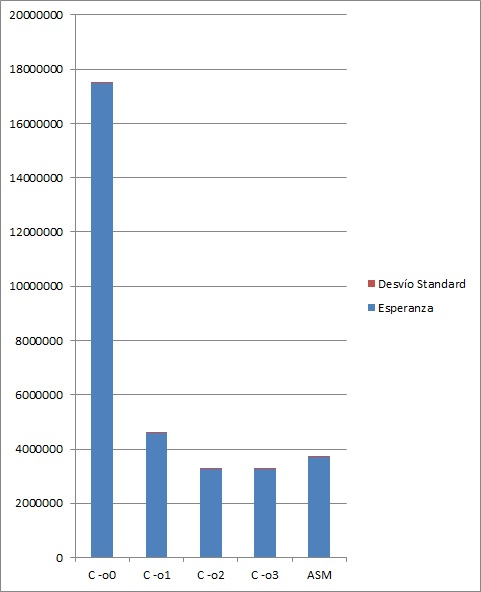
\includegraphics[width=0.6\textwidth]{imagenes/32.jpg}
  \end{center}
\end{figure}

Aqu\'i tambi\'en el valor del desv\'io est\'andar es despreciable. En este caso, podemos notar una vez m\'as que el comando -o0 no ejerce ninguna optimizaci\'on para este programa, ya que es el que tiene mayor tiempo de ejecuci\'on. Bajo el flag -o1 presenta una mejor\'ia, pero sigue requiriendo un tiempo mayor que el programa en Lenguaje Assembler para su ejecuci\'on. Sin embargo, sucede algo llamativo que es que corriendo el lenguaje en lenguaje C tanto bajo el flag -o2 como para -o3 present\'o una esperanza menor que el c\'odigo en Assembler. Asumimos que ocurre esto porque estos flags est\'an dise\~nados para casos como este, donde ensamblan un c\'odigo fuente mejor que el nuestro en Assembler.


% ------------------------------------------------------------------------------
\newpage
\subsection{Filtro \textit{Motion Blur}}
Programar el filtro \textit{mblur} en lenguaje C y en ASM haciendo uso de 
las instrucciones \textbf{SSE}.

% ******************************************************************************
\vspace*{0.3cm} \noindent
\textbf{Experimento 4.1}

Repetir el experimento 1.4 para este filtro \\
\\
El siguiente gr\'afico indica la esperanza de la cantidad de ciclos de clock que toma ejecutar el filtro Bandas en ASM y en C variando los flags de o0 a o3. \\
Reflejando las siguientes magnitudes: \\
\\
 \begin{tabular}[c]{|c|c|c|}
	\hline
		 & Esperanza & Desv\'io est\'andar\\
		\hline
C -o0 & 24.652.732,5 & 117,738 \\
\hline
C -o1 & 11.562.261 & 103,024  \\
\hline
C -o2 & 9.641.346 & 78,159  \\
\hline
C -o3 & 9.639.625 & 78,227 \\
\hline
ASM & 2.993.980,5 & 118,245 \\
\hline
	\end{tabular}\\\\
\\

\begin{figure}[h!]
  \begin{center}
	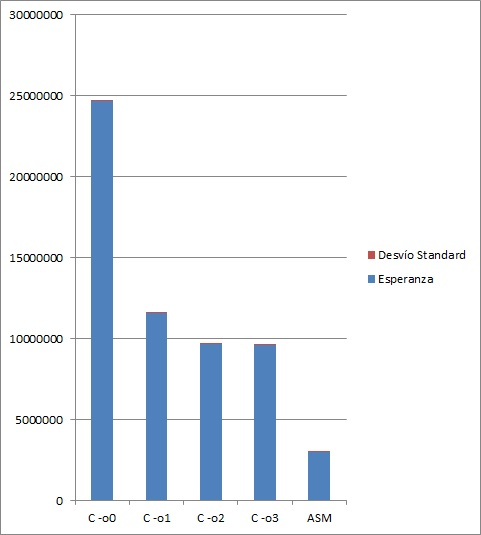
\includegraphics[width=0.7\textwidth]{imagenes/41.jpg}
  \end{center}
\end{figure}
Aqu\'i tambi\'en el valor del desv\'io est\'andar es despreciable. Donde las optimizaciones del compilador en la versi\'on -o3 y la versi\'on -o2 no son suficientes para tener una esperanza menor a la esperanza obtenida bajo el c\'odigo Assembler.\\

\newpage